\chapter{दूसरा नियम: एन्ट्रॉपी}\label{ch:b1:second-law-entropy}

कोई गरम चम्मच ठंडे पानी के प्याले में डालिए: चम्मच ठंडा होता है, पानी गरम,
और दोनों एक ही ताप पर आकर ठहर जाते हैं। पहला नियम उलटा भी उतनी ही आसानी से
होने देता --- पानी और ठंडा होता जाए जबकि चम्मच गरम होता जाए, ऊर्जा जूल भर
तक संरक्षित --- फिर भी ऐसा कभी नहीं होता। उलटी चलाई गई कोई फ़िल्म तुरंत
पहचान में आ जाती है; अणु ऐसे नियम मानते हैं जिनमें कोई दिशा-तीर नहीं, और
संसार में एक तीर है। \omterm{thm:b1:second-law-entropy:secondlaw}{ऊष्मागतिकी का दूसरा नियम} उस राशि को नाम देता है जो
दोनों दिशाओं में भेद करती है: एन्ट्रॉपी, जिसे कोई \omterm{def:b1:newton-dynamics:conservation}{संवृत निकाय} केवल सृजित
कर सकता है, नष्ट कभी नहीं। यह अध्याय उस नियम को बताता है, इस खंड के
निकायों के लिए एन्ट्रॉपी निकालता है, दिखाता है कि वह अनुत्क्रमणीयता को कैसे
मापती है, और अंत में उसे गिनती के रूप में उसका अर्थ देता है।

\begin{omfigure}
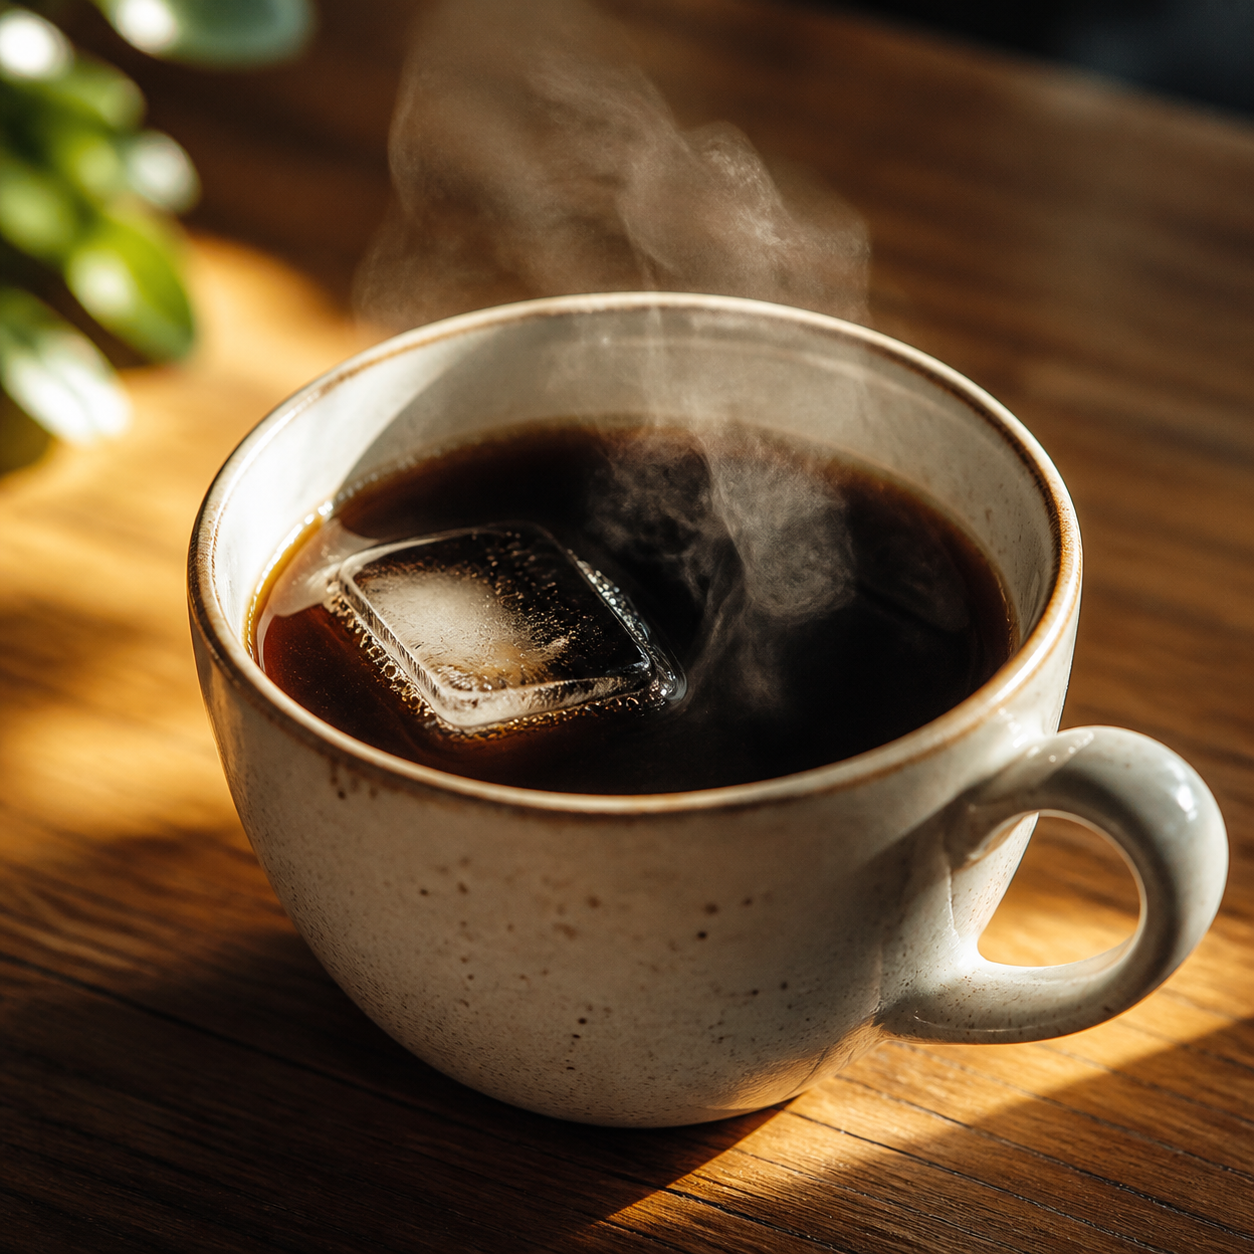
\includegraphics[width=0.42\linewidth]{images/book3/ai/b3-23-coffee-ice-cube.png}

{\small गरम कॉफ़ी में गलता बर्फ़ का टुकड़ा: ऊष्मा केवल एक ही ओर बहती है, और सृजित एन्ट्रॉपी नापती है कि यह मिश्रण उत्क्रमणीय से कितना दूर है।}
\end{omfigure}

\section{दूसरा नियम}

\begin{theorem}[ऊष्मागतिकी का दूसरा नियम]\label{thm:b1:second-law-entropy:secondlaw}
\index{ऊष्मागतिकी का दूसरा नियम}\index{एन्ट्रॉपी}\index{एन्ट्रॉपी!सृजित}\index{एन्ट्रॉपी!विनिमयित}
हर \omterm{def:b1:newton-dynamics:conservation}{संवृत निकाय} के पास एक विस्तीर्ण अवस्था फलन होता है, उसकी
\emph{एन्ट्रॉपी} $S$ (\unit{J/K}), जिससे किसी भी रूपांतरण में
\[
\Delta S = S_{\mathrm{exch}} + S_{\mathrm{created}}, \qquad
S_{\mathrm{exch}} = \int\frac{\delta Q}{T_{\mathrm{ext}}}, \qquad
S_{\mathrm{created}} \geq 0 ,
\]
जहाँ $\delta Q$ वह ऊष्मा है जो परिवेश से उस जगह के ताप
$T_{\mathrm{ext}}$ पर मिलती है जहाँ से वह भीतर आती है, और
$S_{\mathrm{created}} = 0$ तभी और केवल तभी होता है जब रूपांतरण
उत्क्रमणीय हो। किसी विलगित निकाय ($\delta Q = 0$) की एन्ट्रॉपी केवल बढ़
सकती है, और उसका साम्य अधिकतम एन्ट्रॉपी वाली अवस्था होती है।
\end{theorem}
\admitted

\begin{remark}[नियम को पढ़ना]\label{rem:b1:second-law-entropy:reading}
ऊर्जा के विपरीत, एन्ट्रॉपी संरक्षित नहीं रहती: उसका ऊष्मा के साथ
\emph{आदान-प्रदान} होता है (और केवल ऊष्मा के साथ --- कार्य कोई एन्ट्रॉपी
नहीं ढोता), और हर अनुत्क्रमणीय प्रक्रिया उसे \emph{सृजित} करती है: घर्षण,
ताप के अंतर के पार बहती ऊष्मा, निर्वात में लपकती गैस, मिश्रण। सृजित पद ही
अनुत्क्रमणीयता का माप है, और कोई रूपांतरण तभी संभव है जब वह अऋणात्मक हो।
``उत्क्रमणीय'' एक आदर्शीकरण है --- अर्ध-स्थैतिक, घर्षणरहित, लुप्त होते
ताप-अंतरों के पार ऊष्मा का आदान-प्रदान --- जिसके पास वास्तविक प्रक्रियाएँ
पहुँचती तो हैं, पर उस तक कभी नहीं आतीं।
\end{remark}

\begin{omfigure}
\begin{tikzpicture}[font=\small, x=1cm, y=1cm]
  \draw[thick, rounded corners, fill=omDef!8] (0,0) rectangle (4.2,2.6);
  \node at (2.1,1.9) {निकाय};
  \node[omDef] at (2.1,1.15) {$\Delta S = S_{\mathrm{exch}} + S_{\mathrm{created}}$};
  \node[omThm, font=\footnotesize] at (2.1,0.5) {$S_{\mathrm{created}} \geq 0$ (भीतर)};
  \draw[-Stealth, omProp, very thick] (-3.6,1.1) -- (-0.1,1.1) node[midway, above] {$\delta Q$, $T_{\mathrm{ext}}$ पर};
  \node[omProp, font=\footnotesize] at (-1.85,0.65) {$S_{\mathrm{exch}} = \int\delta Q/T_{\mathrm{ext}}$};
  \draw[-Stealth, omExo, very thick] (-3.6,2.2) -- (-0.1,2.2) node[midway, above] {$W$ (कोई एन्ट्रॉपी नहीं)};
\end{tikzpicture}

{\small एन्ट्रॉपी का संतुलन: ऊष्मा सीमा के पार एन्ट्रॉपी $\delta Q/T_{\mathrm{ext}}$
लाती है, कार्य कुछ नहीं लाता, और भीतर की अनुत्क्रमणीय प्रक्रियाएँ कुछ
सृजित करती हैं --- नष्ट कभी नहीं।}
\end{omfigure}

\begin{proposition}[मूल तत्समक; आदर्श गैस और संघनित प्रावस्थाओं की एन्ट्रॉपी]\label{prop:b1:second-law-entropy:identity}
\index{ऊष्मागतिकी का मूल तत्समक}\index{एन्ट्रॉपी!आदर्श गैस की}
नियत संघटन वाले किसी \omterm{def:b1:newton-dynamics:conservation}{संवृत निकाय} के लिए, किसी भी उत्क्रमणीय पथ के अनुदिश,
$\delta Q_{\mathrm{rev}} = T\,\dd S$ और $\delta W_{\mathrm{rev}} = -P\,\dd V$, अतः
\[
\dd U = T\,\dd S - P\,\dd V ,
\]
यानी अवस्था फलनों के बीच एक ऐसा संबंध जो किसी भी अत्यल्प परिवर्तन के लिए
लागू रहता है। फलस्वरूप, \omterm{def:b1:kinetic-theory:model}{आदर्श गैस} के $n$ मोलों के लिए,
\[
S(T, V) = nC_{V,m}\ln T + nR\ln V + \text{अचर}, \qquad
S(T, P) = nC_{P,m}\ln T - nR\ln P + \text{अचर},
\]
और $C$ ऊष्मा धारिता की किसी \omterm{prop:b1:kinetic-theory:condensed}{संघनित प्रावस्था} के लिए, $S(T) = C\ln T + \text{अचर}$।
\end{proposition}

\begin{proof}
उत्क्रमणीय में: $T_{\mathrm{ext}} = T$ और $S_{\mathrm{created}} = 0$ से $\dd S =
\delta Q/T$; फिर पहला नियम वह तत्समक दे देता है, जो अब किसी पथ का उल्लेख
नहीं करता। \omterm{def:b1:kinetic-theory:model}{आदर्श गैस}: $\dd S = (\dd U + P\,\dd V)/T = nC_{V,m}\dd T/T
+ nR\,\dd V/V$; समाकलित कीजिए; और दूसरे रूप के लिए $PV = nRT$ लीजिए।
\omterm{prop:b1:kinetic-theory:condensed}{संघनित प्रावस्था}: $\dd V = 0$, $\dd S = C\,\dd T/T$।
\end{proof}

\begin{example}[सूत्रों को पढ़ना]\label{ex:b1:second-law-entropy:formulas}
कोई रुद्धोष्म \omterm{def:b1:first-law:transformation}{उत्क्रमणीय रूपांतरण} \emph{समएन्ट्रॉपी} होता है: $S(T, V)$ के
अचर रहने से $T^{C_{V,m}}V^R$ अचर मिलता है, अर्थात् $TV^{\gamma - 1}$ अचर ---
यानी फिर से \omterm{prop:b1:first-law:transformations}{लाप्लास का नियम}। अचर ताप पर गैस के किसी \omterm{def:b1:kinetic-theory:scales}{मोल} का आयतन दुगुना
करने से उसकी एन्ट्रॉपी $R\ln2 = \qty{5.8}{J/K}$ बढ़ जाती है, चाहे यह
उत्क्रमणीय ढंग से किया जाए (एन्ट्रॉपी ऊष्मा-भंडार से ऊष्मा के रूप में आती
है) या निर्वात में \omterm{rem:b1:first-law:irreversible}{जूल प्रसार} से (कोई ऊष्मा नहीं: तब वही \qty{5.8}{J/K}
\emph{सृजित} होती है)। अवस्था फलन को इससे कोई मतलब नहीं कि वह वहाँ
पहुँचा कैसे; संतुलन को है।
\end{example}

\section{एन्ट्रॉपी के संतुलन}

\begin{proposition}[ऊष्मा-भंडार के साथ ऊष्मा का आदान-प्रदान]\label{prop:b1:second-law-entropy:thermostat}
जो निकाय ऊष्मा $Q$ किसी ऐसे ऊष्मा-भंडार से पाता है जो $T_0$ पर हो (भीतर
चाहे कुछ भी होता रहे), उसका $S_{\mathrm{exch}} = Q/T_0$ होता है, और ऊष्मा-भंडार की अपनी
एन्ट्रॉपी $-Q/T_0$ से बदलती है: यानी ऊष्मा-भंडार एन्ट्रॉपी का आदान-प्रदान
उत्क्रमणीय ढंग से करता है।
\end{proposition}

\begin{proof}
$T_{\mathrm{ext}} = T_0$ अचर है; ऊष्मा-भंडार की अपनी आंतरिक अवस्था अत्यल्प
बदलती है, अतः उसका अपना सृजन नगण्य रहता है।
\end{proof}

\begin{example}[ठंडी झील में गरम पिंड]\label{ex:b1:second-law-entropy:quench}
लोहे का कोई गुटका ($m = \qty{1.0}{kg}$, $c = \qty{450}{J/(kg.K)}$), जो $T_1 =
\qty{373}{K}$ पर हो, $T_0 = \qty{293}{K}$ की किसी झील में डाला जाता है: वह $T_0$ पर आकर ठहरता है,
जहाँ $\Delta S_{\text{गुटका}} = mc\ln(T_0/T_1) = \qty{-109}{J/K}$ और झील को दी गई $Q =
mc(T_0 - T_1) = \qty{-36}{kJ}$, अतः $S_{\mathrm{exch}} =
Q/T_0 = \qty{-123}{J/K}$ और $S_{\mathrm{created}} = -109 + 123 = \qty{+14}{J/K}$।
गुटके की एन्ट्रॉपी घटी, झील की उससे अधिक बढ़ी: यानी प्रक्रिया
अनुत्क्रमणीय है, और वह संख्या नापती है कि कितनी।
\end{example}

\begin{proposition}[दो परिणाम]\label{prop:b1:second-law-entropy:clausiuskelvin}
\index{क्लॉज़ियस का कथन}\index{केल्विन का कथन}
\begin{enumerate}
  \item \emph{(क्लॉज़ियस)} ऊष्मा किसी ठंडे पिंड से किसी अधिक गरम पिंड की
        ओर अपने आप नहीं बहती: कोई राशि $Q > 0$, जो $T_h$ से
        $T_c < T_h$ तक जाए, $S = Q(1/T_c - 1/T_h) > 0$ सृजित करती है; और उलटा
        एन्ट्रॉपी नष्ट कर देता।
  \item \emph{(\omterm{def:b1:kinetic-theory:temperature}{केल्विन})} कोई चक्रीय मशीन किसी एक ही ऊष्मा-भंडार से कार्य
        नहीं बना सकती: किसी चक्र पर $\Delta S = 0 = Q/T_0 + S_{\mathrm{created}}$
        से $Q \leq 0$ बाध्य हो जाता है, अतः $W = -Q \geq 0$ --- यानी मशीन
        केवल कार्य \emph{ले} सकती है और ऊष्मा छोड़ सकती है।
\end{enumerate}
\end{proposition}

\begin{proof}
दोनों वही संतुलन हैं, जो ``दोनों ऊष्मा-भंडार'' या ``पूरे चक्र पर मशीन''
वाले निकाय पर लगाया गया है, जहाँ $S$ अवस्था फलन है, और इसलिए किसी चक्र पर $\Delta S
= 0$ रहता है।
\end{proof}

\begin{definition}[एन्ट्रॉपी आरेख]\label{def:b1:second-law-entropy:TS}
\index{एन्ट्रॉपी आरेख}
$(S, T)$ तल में कोई \omterm{def:b1:first-law:transformation}{उत्क्रमणीय रूपांतरण} एक वक्र होता है, और मिली ऊष्मा उसके
नीचे का क्षेत्रफल: $Q_{\mathrm{rev}} = \int T\,\dd S$। कोई उत्क्रमणीय समतापी
वक्र क्षैतिज होता है, और कोई समएन्ट्रॉपी (उत्क्रमणीय रुद्धोष्म) वक्र
ऊर्ध्वाधर; और कोई उत्क्रमणीय चक्र उतना क्षेत्रफल घेरता है जितनी उसे मिली
ऊष्मा है, और इसलिए, पहले नियम से, जितना उसने कार्य दिया
(\cref{ch:b1:heat-engines})।
\end{definition}

\begin{omfigure}
\begin{tikzpicture}
\begin{axis}[omaxis, axis x line=bottom, axis y line=left, width=8.4cm, height=5.6cm, xlabel={$S$}, ylabel={$T$},
    xlabel style={at={(axis description cs:0.5,-0.08)}, anchor=north},
    xmin=0, xmax=5, ymin=0, ymax=4.2, xtick={1,3.5}, xticklabels={$S_1$,$S_2$}, ytick={1.2,3.2}, yticklabels={$T_c$,$T_h$}]
  \fill[omExo!20] (axis cs:1,0) rectangle (axis cs:3.5,3.2);
  \draw[omThm, thick] (axis cs:1,3.2) -- (axis cs:3.5,3.2);
  \draw[omDef, thick] (axis cs:3.5,3.2) -- (axis cs:3.5,1.2);
  \draw[omThm, thick] (axis cs:3.5,1.2) -- (axis cs:1,1.2);
  \draw[omDef, thick] (axis cs:1,1.2) -- (axis cs:1,3.2);
  \fill[white] (axis cs:1,0) rectangle (axis cs:3.5,1.2);
  \fill[omExo!35] (axis cs:1,1.2) rectangle (axis cs:3.5,3.2);
  \node[font=\footnotesize] at (axis cs:2.25,2.2) {दिया गया $W$};
  \node[omThm, font=\footnotesize, above] at (axis cs:2.25,3.25) {$Q_h = T_h\Delta S$};
  \node[omThm, font=\footnotesize, below] at (axis cs:2.25,1.15) {$\abs{Q_c} = T_c\Delta S$};
\end{axis}
\end{tikzpicture}\qquad
\begin{tikzpicture}
\begin{axis}[omaxis, axis x line=bottom, axis y line=left, width=7.0cm, height=5.6cm, xlabel={$T_1/T_2$}, ylabel={$S_{\mathrm{created}}/mc$},
    xlabel style={at={(axis description cs:0.5,-0.1)}, anchor=north},
    xmin=0, xmax=4.2, ymin=0, ymax=0.6, xtick={1,2,3,4}, ytick={0.2,0.4}]
  \addplot[omDef, thick, domain=0.15:4.2, samples=200] {ln((1+x)^2/(4*x))};
  \node[omDef, font=\footnotesize] at (axis cs:2.6,0.45) {$\ln\dfrac{(T_1 + T_2)^2}{4T_1T_2}$};
\end{axis}
\end{tikzpicture}

{\small बाएँ: \omterm{def:b1:second-law-entropy:TS}{एन्ट्रॉपी आरेख} में दो समतापी और दो समएन्ट्रॉपी वक्रों वाला
कोई उत्क्रमणीय चक्र गरम ताप पर $T_h\Delta S$ लेता है, ठंडे पर
$T_c\Delta S$ छोड़ता है, और अंतर को कार्य के रूप में दे देता है --- यानी
अगले अध्याय का कार्नो चक्र। दाएँ: $T_1$ और $T_2$ पर के दो बराबर पिंडों को
संस्पर्श में लाने पर सृजित एन्ट्रॉपी: केवल $T_1 = T_2$ के लिए शून्य, और
अन्यथा धनात्मक।}
\end{omfigure}

\begin{method}[एन्ट्रॉपी का संतुलन बनाना]\label{met:b1:second-law-entropy:method}
\begin{enumerate}
  \item अवस्था फलनों से निकाय का $\Delta S$ निकालिए
        (\cref{prop:b1:second-law-entropy:identity}): केवल आरंभिक और
        अंतिम अवस्थाओं से।
  \item वास्तव में मिली ऊष्मा और स्रोत के ताप से $S_{\mathrm{exch}}$
        निकालिए: ऊष्मा-भंडारों के लिए $\sum Q_i/T_i$, और अन्यथा
        $\int\delta Q/T_{\mathrm{ext}}$।
  \item इससे $S_{\mathrm{created}} = \Delta S - S_{\mathrm{exch}}$ निकालिए; वह
        $\geq 0$ होना ही चाहिए --- न हो तो रूपांतरण असंभव है (या कहीं भूल
        हुई है); और उत्क्रमणीय के लिए $= 0$।
\end{enumerate}
\end{method}

\begin{example}[गरम और ठंडे का मिश्रण]\label{ex:b1:second-law-entropy:mixing}
पानी के दो बराबर द्रव्यमान $m$, जो $T_1$ और $T_2$ पर हों, किसी तापरोधी
पात्र में मिलाने पर $(T_1 + T_2)/2$ पर आकर ठहरते हैं (पहला नियम); $\Delta S = mc[\ln\frac{T_f}{T_1} + \ln\frac{T_f}{T_2}]
= mc\ln\frac{(T_1 + T_2)^2}{4T_1T_2} \geq 0$ (समांतर माध्य गुणोत्तर माध्य से
बड़ा होता है), और कोई आदान-प्रदान नहीं: यानी सब सृजित। \qty{300}{K} और
\qty{400}{K} पर \qty{1}{kg} के लिए: \qty{86}{J/K}। सप्ताहांत समस्या दिखाती
है कि उन्हें \emph{उत्क्रमणीय} ढंग से --- किसी आदर्श इंजन के ज़रिए ---
मिलाने पर उलटे कार्य मिल जाता और वे $\sqrt{T_1T_2}$ पर आकर ठहरते।
\end{example}

\section{एन्ट्रॉपी गिनती क्या है}

\begin{proposition}[बोल्ट्ज़मान का सूत्र]\label{prop:b1:second-law-entropy:boltzmann}
\index{बोल्ट्ज़मान का सूत्र}\index{सूक्ष्म-अवस्था}
कोई स्थूल अवस्था (दिए हुए $U$, $V$, $N$ के साथ) सूक्ष्म विन्यासों
(\emph{सूक्ष्म-अवस्थाओं}) की किसी संख्या $\Omega$ से साकार हो सकती है।
उसकी एन्ट्रॉपी यह है
\[
S = k_B\ln\Omega .
\]
कोई विलगित निकाय उसी स्थूल अवस्था की ओर विकसित होता है जिसके पास कहीं
अधिक सूक्ष्म-अवस्थाएँ हों: एन्ट्रॉपी का बढ़ना उसी अत्यंत प्रबल संभावना की
ओर का कूच है।
\end{proposition}
\admitted

\begin{example}[गैस लौटकर क्यों नहीं आती]\label{ex:b1:second-law-entropy:count}
किसी डिब्बे के किसी भी आधे भाग में रहने को स्वतंत्र $N$ अणु: $2^N$
व्यवस्थाएँ, सब समान रूप से संभाव्य; और उनमें से केवल एक में सब बाईं ओर
होते हैं। किसी आधे भाग में बंद गैस को फैलने देने पर $\Omega$ $2^N$ से गुणा
हो जाता है, अतः $\Delta S =
Nk_B\ln2 = nR\ln2$ --- यानी ठीक ऊपर वाला जूल-प्रसार का परिणाम, पर अब एक
अर्थ के साथ: अणुओं के पास होने के $2^N$ गुना अधिक तरीके हैं। उनके अपने आप
लौट आने की संभावना $2^{-N}$ है: दस अणुओं के लिए हज़ार में एक, सौ के लिए
$10^{30}$ में एक, और किसी \omterm{def:b1:kinetic-theory:scales}{मोल} के लिए $10^{23}$ शून्यों वाली कोई संख्या।
दूसरा नियम कोई निषेध नहीं है; वह इतनी एकतरफ़ा संभावना है कि उसे एक बार भी
विफल होते नहीं पकड़ा गया।
\end{example}

\begin{omfigure}
\begin{tikzpicture}
\begin{axis}[omaxis, axis x line=bottom, axis y line=left, width=9.5cm, height=5.2cm, xlabel={बाईं ओर के अणु, $k$}, ylabel={व्यवस्थाओं की संख्या},
    xlabel style={at={(axis description cs:0.5,-0.16)}, anchor=north},
    scaled y ticks=false,
    xmin=-0.7, xmax=20.7, ymin=0, ymax=2.05e5, xtick={0,5,10,15,20}, ytick={1e5,2e5}, yticklabels={$10^5$,$2\times10^5$},
    ybar, bar width=5pt]
  \addplot[fill=omDef!40, draw=omDef] coordinates {(0,1) (1,20) (2,190) (3,1140) (4,4845) (5,15504) (6,38760) (7,77520) (8,125970) (9,167960) (10,184756) (11,167960) (12,125970) (13,77520) (14,38760) (15,15504) (16,4845) (17,1140) (18,190) (19,20) (20,1)};
  \node[font=\footnotesize, omDef] at (axis cs:15.5,1.5e5) {$N = 20$: $\binom{20}{k}$};
  \draw[omThm, -Stealth] (axis cs:0.8,1.2e5) -- (axis cs:0.2,8e3);
  \node[font=\footnotesize, omThm, anchor=west] at (axis cs:0.1,1.35e5) {सब बाईं ओर: $1$};
\end{axis}
\end{tikzpicture}

{\small किसी डिब्बे में बीस अणु: उन व्यवस्थाओं की संख्या जिनमें उनमें से
$k$ बाएँ आधे भाग में हों। बराबर बँटवारा $184756$ तरीकों से साकार होता है,
और सब-बाईं-ओर वाली अवस्था केवल एक तरीके से। $10^{23}$ अणुओं के साथ वह
शिखर $10^{-11}$ सापेक्ष चौड़ाई की एक कील बन जाता है: एकसमान गैस कोई नियम
नहीं, वह अकेली चीज़ है जिसे कभी देखा जा सकता है।}
\end{omfigure}

\section{अभ्यास}

\begin{exercise}[$\star$]\label{exo:b1:second-law-entropy:1}
\qty{0}{\degreeCelsius} पर गलती \qty{1.0}{kg} बर्फ़ की
($L_f = \qty{334}{kJ/kg}$), और \qty{100}{\degreeCelsius} पर उबलते
\qty{1.0}{kg} पानी की ($L_v = \qty{2260}{kJ/kg}$) एन्ट्रॉपी में परिवर्तन।
दूसरा इतना बड़ा क्यों है?
\end{exercise}

\begin{exercise}[$\star$]\label{exo:b1:second-law-entropy:2}
\qty{20}{} से \qty{80}{\degreeCelsius} तक गरम किए गए \qty{1.0}{kg} पानी की
एन्ट्रॉपी में परिवर्तन। क्या वह इस पर निर्भर करता है कि गरम कैसे किया गया?
\end{exercise}

\begin{exercise}[$\star$]\label{exo:b1:second-law-entropy:3}
\omterm{def:b1:kinetic-theory:model}{आदर्श गैस} का एक \omterm{def:b1:kinetic-theory:scales}{मोल} अचर ताप पर अपना आयतन दुगुना कर लेता है।
$\Delta S$; और प्रसार के उत्क्रमणीय होने पर तथा निर्वात में \omterm{rem:b1:first-law:irreversible}{जूल प्रसार} होने
पर आदान-प्रदान की गई और सृजित एन्ट्रॉपी।
\end{exercise}

\begin{exercise}[$\star$]\label{exo:b1:second-law-entropy:4}
$S(T, V)$ से दिखाइए कि किसी \omterm{def:b1:kinetic-theory:model}{आदर्श गैस} का कोई उत्क्रमणीय \omterm{prop:b1:first-law:transformations}{रुद्धोष्म रूपांतरण}
$TV^{\gamma - 1} =$ अचर मानता है। किसी \emph{अचानक} किए गए रुद्धोष्म संपीडन
(\cref{exo:b1:first-law:11}) में एन्ट्रॉपी का परिवर्तन क्या होता है?
उसी अभ्यास के आँकड़ों के लिए उसे निकालिए।
\end{exercise}

\begin{exercise}[$\star\star$]\label{exo:b1:second-law-entropy:5}
\qty{100}{\degreeCelsius} पर लोहे का \qty{1.0}{kg} का कोई गुटका ($c = \qty{450}{J/(kg.K)}$)
\qty{20}{\degreeCelsius} की किसी झील में डाला जाता है। गुटके की, झील की और
विश्व की एन्ट्रॉपी में परिवर्तन।
\end{exercise}

\begin{exercise}[$\star\star$]\label{exo:b1:second-law-entropy:6}
\qty{300}{K} और \qty{400}{K} पर पानी के दो \qty{1.0}{kg} द्रव्यमान
रुद्धोष्म रूप से मिलाए जाते हैं। अंतिम ताप, सृजित एन्ट्रॉपी। सामान्य रूप
से दिखाइए कि सृजित एन्ट्रॉपी $mc\ln[(T_1 + T_2)^2/4T_1T_2]$ अऋणात्मक है।
\end{exercise}

\begin{exercise}[$\star\star$]\label{exo:b1:second-law-entropy:7}
\qty{1.0}{kJ} का ऊष्मा-रिसाव \qty{300}{K} के किसी कमरे से किसी दीवार के पार
\qty{280}{K} के बाहर जाता है। सृजित एन्ट्रॉपी। वही ऊष्मा \qty{1000}{K} की
किसी भट्ठी से कमरे तक: तुलना कीजिए, और टिप्पणी कीजिए कि ``हानि'' सबसे
अधिक कहाँ है।
\end{exercise}

\begin{exercise}[$\star\star$]\label{exo:b1:second-law-entropy:8}
किसी एक ऊष्मा-भंडार के संस्पर्श में चक्र चलाती किसी मशीन के एन्ट्रॉपी-संतुलन
से \omterm{prop:b1:second-law-entropy:clausiuskelvin}{केल्विन का कथन} सिद्ध कीजिए। किसी जहाज़ का इंजन ऊष्मा सीधे समुद्र से
क्यों नहीं खींच लेता?
\end{exercise}

\begin{exercise}[$\star\star$]\label{exo:b1:second-law-entropy:9}
एक ही $T$ और $P$ पर नाइट्रोजन का एक \omterm{def:b1:kinetic-theory:scales}{मोल} और ऑक्सीजन का एक \omterm{def:b1:kinetic-theory:scales}{मोल}, जो कुल आयतन
$2V$ के किसी डिब्बे में किसी दीवार से अलग रखे हों, मिलने दिए जाते हैं।
एन्ट्रॉपी में परिवर्तन (हर गैस को पूरे डिब्बे में फैलता मानिए)। वह सृजित है
या आदान-प्रदान की गई? और यदि दोनों ओर नाइट्रोजन ही होती तो?
\end{exercise}

\begin{exercise}[$\star\star\star$]\label{exo:b1:second-law-entropy:10}
\qty{100}{W} का कोई बल्ब एक घंटे जलता है; उसकी सारी ऊर्जा अंत में
\qty{293}{K} के किसी कमरे में ऊष्मा बन जाती है। सृजित एन्ट्रॉपी। वह,
भौतिक रूप से, सृजित कहाँ हुई?
\end{exercise}

\begin{exercise}[$\star\star\star$]\label{exo:b1:second-law-entropy:11}
$C$ ऊष्मा धारिता का कोई पिंड, जो $T_1$ पर है, $T_0 < T_1$ तक ठंडा किया जाता
है: (क) $T_0$ पर के किसी ऊष्मा-भंडार से सीधे संस्पर्श द्वारा, (ख)
$\sqrt{T_1T_0}$ पर के किसी बीच के ऊष्मा-भंडार से होकर दो चरणों में, (ग)
ऊष्मा-भंडारों की किसी संततता से होकर। हर स्थिति में सृजित एन्ट्रॉपी; और
निष्कर्ष निकालिए कि ``उत्क्रमणीय शीतलन'' के लिए क्या चाहिए होगा।
\end{exercise}

\begin{exercise}[$\star\star\star$]\label{exo:b1:second-law-entropy:12}
यह प्रायिकता कि $N$ अणु सब-के-सब डिब्बे के बाएँ आधे भाग में बैठे हों,
$N = 10$, $100$, $10^{22}$ के लिए (अंतिम को दस की घात के रूप में लिखिए)।
दिखाइए कि $\Delta S = k_B\ln(2^N)$ का मान $nR\ln2$ के बराबर है, और
``अनुत्क्रमणीय'' तथा ``असंभव'' शब्दों पर टिप्पणी कीजिए।
\end{exercise}

\section{समस्या: कॉफ़ी का प्याला और समय का तीर}

\begin{problem}[{सप्ताहांत समस्या --- ठंडा होता एक प्याला, मिलाया गया एक
जल-कुंड, एक प्रशीतक और अणुओं का एक डिब्बा: चार एन्ट्रॉपी-संतुलन, और सृजित
एन्ट्रॉपी कार्य के रूप में कितनी क़ीमत की थी}]
\label{pb:b1:second-law-entropy:1}
पानी: $c = \qty{4180}{J/(kg.K)}$; कमरा (एक ऊष्मा-भंडार): $T_0 = \qty{293}{K}$;
$R = \qty{8.314}{J/(mol.K)}$, $k_B = \qty{1.38e-23}{J/K}$।

\medskip
\noindent\textbf{भाग I --- ठंडा होता प्याला।}
\qty{0.25}{kg} कॉफ़ी का कोई प्याला, जो $T_1 = \qty{363}{K}$ पर है, कमरे के
ताप तक ठंडा होता है।
\begin{enumerate}
  \item कमरे को दी गई ऊष्मा, और कमरे की एन्ट्रॉपी में परिवर्तन।
  \item कॉफ़ी की एन्ट्रॉपी में परिवर्तन।
  \item सृजित एन्ट्रॉपी; उसका चिह्न जाँचिए।
  \item प्याला \qty{330}{K} पर पहुँचते ही पी लिया जाता है: उस क्षण तक
        सृजित एन्ट्रॉपी।
  \item दिखाइए कि किसी भी $T_1 > T_0$ के लिए $S_{\mathrm{created}} = mc[T_1/T_0 - 1 -
        \ln(T_1/T_0)] \geq 0$ ($f(x) = x - 1 - \ln x$ का अध्ययन कीजिए)।
  \item हिलाने या फूँक मारने पर कॉफ़ी तेज़ी से ठंडी होती है: क्या इससे
        सृजित एन्ट्रॉपी बदलती है? क्यों, या क्यों नहीं?
\end{enumerate}

\medskip
\noindent\textbf{भाग II --- मिलाना, बुरी तरह और भली तरह।}
किसी तापरोधी पात्र में, $T_1 = \qty{400}{K}$ और $T_2 =
\qty{300}{K}$ पर पानी के दो \qty{1.0}{kg} द्रव्यमान।
\begin{enumerate}[resume]
  \item सीधा मिश्रण: अंतिम ताप $T_f$ और सृजित एन्ट्रॉपी।
  \item इसके बदले, कोई आदर्श इंजन गरम पानी से ऊष्मा लेता है, ठंडे को
        ऊष्मा छोड़ता है और कार्य देता है, जब तक दोनों एक ही ताप
        $T_f'$ पर न आ जाएँ; पूरी प्रक्रिया उत्क्रमणीय है।
        एन्ट्रॉपी-संतुलन लिखिए और दिखाइए कि $T_f' = \sqrt{T_1T_2}$।
  \item $T_f'$ और दिया गया कार्य निकालिए (दोनों पानियों पर पहला नियम)।
  \item उत्क्रमणीय योजना का एन्ट्रॉपी-संतुलन संख्याओं से जाँचिए: गरम पानी
        ने जितनी एन्ट्रॉपी खोई, ठंडे ने उतनी ही पाई।
  \item उस कार्य की तुलना प्रश्न 6 के $T_0 \times S_{\mathrm{created}}$ से
        कीजिए (यहाँ कमरे को संदर्भ ताप मानिए, $T_0 \approx T_2$):
        लापरवाह मिश्रण की सृजित एन्ट्रॉपी क्या नापती है?
  \item कोई रसोई वह कार्य वसूल क्यों नहीं करती?
\end{enumerate}

\medskip
\noindent\textbf{भाग III --- प्रशीतक।}
कोई प्रशीतक अपने भीतर का ताप $T_c = \qty{278}{K}$ बनाए रखता है, उस कमरे
में जो $T_0$ पर है; उसमें \qty{40}{W} से ऊष्मा रिसती है, जिसे मशीन वापस बाहर पंप करती है।
\begin{enumerate}[resume]
  \item एक सेकंड के लिए मशीन (एक चक्रीय युक्ति) का एन्ट्रॉपी-संतुलन
        लिखिए: ठंडे भीतरी भाग से मिली, कमरे को दी गई, और भीतर सृजित
        एन्ट्रॉपी।
  \item इससे प्रति सेकंड न्यूनतम कार्य (यानी \omterm{thm:b1:dc-circuits:kirchhoff}{विद्युत शक्ति}) निकालिए, और
        उससे संगत अधिकतम निष्पादन गुणांक
        $Q_c/W$।
  \item उस सीमा को केवल $T_c$ और $T_0$ के रूप में लिखिए, और $T_c = \qty{255}{K}$
        के किसी हिमकारक के लिए उसका मान निकालिए।
  \item इस आकार का कोई वास्तविक प्रशीतक लगभग \qty{15}{W} खींचता है: प्रति
        सेकंड सृजित एन्ट्रॉपी।
  \item खुला छोड़ने पर प्रशीतक का दरवाज़ा \qty{200}{W} से ऊष्मा भीतर आने
        देता है: अब न्यूनतम शक्ति, और खुला प्रशीतक कमरे को गरम क्यों कर
        देता है।
  \item ऐसे किसी प्रशीतक के बारे में दूसरा नियम क्या कहता, जिसे बिजली की
        ज़रूरत ही न हो?
\end{enumerate}

\medskip
\noindent\textbf{भाग IV --- गिनती।}
किसी डिब्बे को एक दीवार दो बराबर हिस्सों में बाँटती है; \omterm{def:b1:kinetic-theory:model}{आदर्श गैस} के $N$
अणु बाईं ओर हैं। दीवार हटा दी जाती है।
\begin{enumerate}[resume]
  \item पहले और बाद में सूक्ष्म-अवस्थाओं की संख्या (हर अणु किसी भी आधे भाग
        में हो सकता है), और बोल्ट्ज़मान के सूत्र से $\Delta S$।
  \item \omterm{rem:b1:first-law:irreversible}{जूल प्रसार} के लिए ऊष्मागतिक सूत्र से मिलते $\Delta S = nR\ln2$ के
        सामने इसे जाँचिए।
  \item $N = 50$ के लिए, किसी यादृच्छिक क्षण पर सारे अणु फिर से बाईं ओर
        मिलने की प्रायिकता; और किसी एक \omterm{def:b1:kinetic-theory:scales}{मोल} के लिए, उस प्रायिकता की कोटि दस
        की घात के रूप में।
  \item यह बताने के लिए कि $N$ अणुओं में से हर एक किस आधे भाग में है, कितने
        हाँ/नहीं प्रश्न (बिट) चाहिए? $\Delta S/(k_B\ln2)$ से तुलना कीजिए।
  \item \omterm{rem:b1:first-law:irreversible}{जूल प्रसार} में आदान-प्रदान की गई और सृजित एन्ट्रॉपी; वह
        अनुत्क्रमणीयता का पाठ्यपुस्तकीय उदाहरण क्यों है?
  \item वही गैस उत्क्रमणीय और समतापी ढंग से वापस बाएँ आधे भाग तक संपीडित
        की जाती है: मिला कार्य, कमरे को दी गई ऊष्मा, आदान-प्रदान की गई
        एन्ट्रॉपी; मुक्त प्रसार को उलटने के लिए क्या-क्या देना पड़ता है?
  \item तीन पंक्तियों में सार दीजिए: दूसरा नियम क्या संरक्षित रखता है
        (कुछ नहीं), क्या मना करता है, और सृजित एन्ट्रॉपी की क़ीमत क्या है।
\end{enumerate}
\end{problem}
